\section{Positive and Unlabeled Learning}
\label{sec:pulearning}

%%%%%%%% TEXT PU Learning setup
\paragraph{Learning with inexhaustive segmentation fits a PU learning setup}
\noindent \textit{This part should formulate the PU learning probleml and discuss why PU Learning instead of semi-supervised learning is the way to go.}

\noindent
To simplify the demonstration, let us consider a binary segmentation problem where we have \textit{positive} and \textit{negative} pixels denoting pixels corresponding to target and non-target segments.
The goal of compensating incompleteness is to learn a model that predicts as many positive pixels as possible while keeping the false positive rate low.
A pixel with a negative label can be either a truly negative pixel or a wrongly unsegmented positive pixel.
% It will require extra manual works to distinguish the two cases explicitly.
%%%%%%%% TEXT Weighted loss for negatives
\paragraph{Class-weighted Logistic Loss}
\noindent \textit{This part should discuss the difficulty of applying traditional PU learning methods to deep learning and then introduce the idea of re-weigh positive and negative classes.}

\noindent
Our original goal was to achieve high precision as well as high recall regardless the existence of false negative labels.
A straightforward way to achieve this goal is to simply reweigh the positive and negative examples, namely let the positive and negative examples have different rates of contribution to the total loss.
Suppose logistic loss is used, the corresponding losses for positive and negative samples are:
\begin{equation*}
  \begin{aligned}
    & l_{\tilde{y_i}=+1} = - \log p(y_i=+1|x_i) \\
    & l_{\tilde{y_i}=-1} = - q \log p(y_i=-1 \vert x_i), 0<q<1
  \end{aligned}
\end{equation*}
where $p(y_i \vert x_i)=\sigma(f(x))$ denotes the probablistic output of the model $f(\cdot)$ for the i-th example. Emprically, the choice of $q$ can be made based on the most highest precision and recall achieved on validation set.
Alternatively, one can also roughly assign $q=p(y=-1 \vert \tilde{y}=-1)$.
This turns out to be part of the backward corrected loss proposed in \cite{patrini2016making}:
\begin{equation*}
  \begin{aligned}
    l_{\tilde{y_i}=-1} = - p(y_i=-1 \vert \tilde{y_i}=-1) \log p(y_i=-1 \vert x_i) \\ - p(y_i=+1 \vert \tilde{y_i}=-1) \log p(y_i=+1 \vert x_i)
  \end{aligned}
\end{equation*}
% $$p( \tilde{y} \vert x, y) = \sum_{y}p(\tilde{y} \vert y)p(y \vert x)$$
% $$p(y=+1 \vert \tilde{y}=+1) = 1 $$
% $$p(y=-1 \vert \tilde{y}=+1) = 0 $$
with $p(y_i=-1 \vert \tilde{y_i}=-1) = q$ and $p(y_i=+1 \vert \tilde{y_i}=-1) = 1-q$.


%%%%%%%% TEXT Encouraging confident predictions
% \paragraph{Confidence of contrary prediction and probability of false negative label}
% \noindent
% \noindent \textit{The idea of alleviating punishment for confident predictions.}
% Losses above assume that the true label of an observed negative label is independent of the inputs $x$.
% However, the true label $y$ is often dependent on both $x$ and $\tilde{y}$ in practice.
% For instance, in segmentation problems, whether a pixel is left unsegmented correctly or not can be determined by the semantical meaning of this pixel and pixels around.
% It is nevertheless difficult to estimate $p(y \vert x, \tilde{y})$ directly due to the difficulty of exploring the joint distribution of $x$ and $\tilde{y}$.
% Alternatively, one can use the probabilistic prediction $p(y \vert x;\theta)$ a classification model to provide extra information about the inputs.
% The predicted probabilities indicate how confident the current model is for the predictions made.
% Given a good enough model, more confident positive predictions for negatively labeled examples can have a higher probability of being wrongly annotated than the less confident ones.
% \footnote{J: This argument needs more detailed explanation.}
% With a random model by which predictions are made randomly, the high and low confidences do not convey any information about the underlying inputs distribution.
% By contrast, confident predictions made by a trained model indicate that the corresponding samples are possibly close to some previous training samples with positive labels in the feature space.
% The natural trend of similar examples having the same labels supports a higher probability of being annotated wrongly for confident predictions which have opposite labels.
% This thought leads to the idea of not punishing confident contrary predictions more than unconfident ones as the traditional logistic/softmax loss will do.

%%%%%%%% TEXT Exponential loss
\paragraph{Exponential Loss for unlabeled examples}
\noindent
\noindent \textit{This section should mention the class dependent losses and introduce ExponentialUnlabeledLoss}
In a PU learning setup, the positive (P) set contains only reliable positive labels, whereas the unlabeled (U) set can be considered as noisy negative labels.
The problem then converts to training with clean positive examples and noisy negative examples.
We used a class-dependent loss to compensate the noisy negative labels while still making full use of the clean positive labels.
The loss was made of a normal logistic loss for positive examples and an exponential loss \cite{tax2016class} for examples with negative labels:
\begin{equation*}
  \begin{aligned}
    & l_{\tilde{y_i}=+1} = - \log p(y_i=+1 \vert x_i) \\
    & l_{\tilde{y_i}=-1} = 1 - p(y_i=-1|x_i)
  \end{aligned}
\end{equation*}
Figure \ref{fig:losses} shows the weighted logistic loss with $q=0.5$ and the exponential unlabeled loss respectively and their derivatives with respect to logits by varing the logit from negative to positive.
The main feature of exponential loss is its relatively small changes in the region of confident positive for negatively labeled examples, compared to the logistic loss and class weighted logistic loss.
As a consequence of this feature, the corresponding derivative decreases to zero as the prediction increases in the positive direction.
This feature interprets the idea of not punishing positive prediction with confidence for negatively labeled samples.

\noindent \textit{This section discuss the loss and derivative difference between the losses.}
\noindent
Figure \ref{fig:moons} shows the loss and derivate difference between logistic loss, class-weighted logistics loss and exponential negative (unlabeled) loss with a two-dimensional example.
It demonstrates that, for exponential unlabeled loss, unlabeled positive examples farther from the decision boundary do not have larger loss contributions as ones closer to but still distant from the decision boundary.
Confident positive predictions, shown as examples located on the positive side of the decision boundary and far from it, has little effect for updating model weights.
The consequence of this effect is that positive examples push the decision boundary away from the positive cluster while negative examples closed to the decision boundary instead of those away from the decision boundary pull the decision boundary towards the positive cluster.
This characterisitc of exponential loss lead to a selectively counting weights update contributions of negative samples than simply lower the overall estimation for all negative samples while optimization.
The exponential loss was introduced in \cite{tax2016class} to get rid of the effect of outliers.
In our case, the negative examples given confident predictions by classifier can be considered as outliers.

%%%%%%%% FIGURE Losses
\begin{figure}[t]
\centering
% \fbox{\rule{0pt}{2in} \rule{0.9\linewidth}{0pt}}
   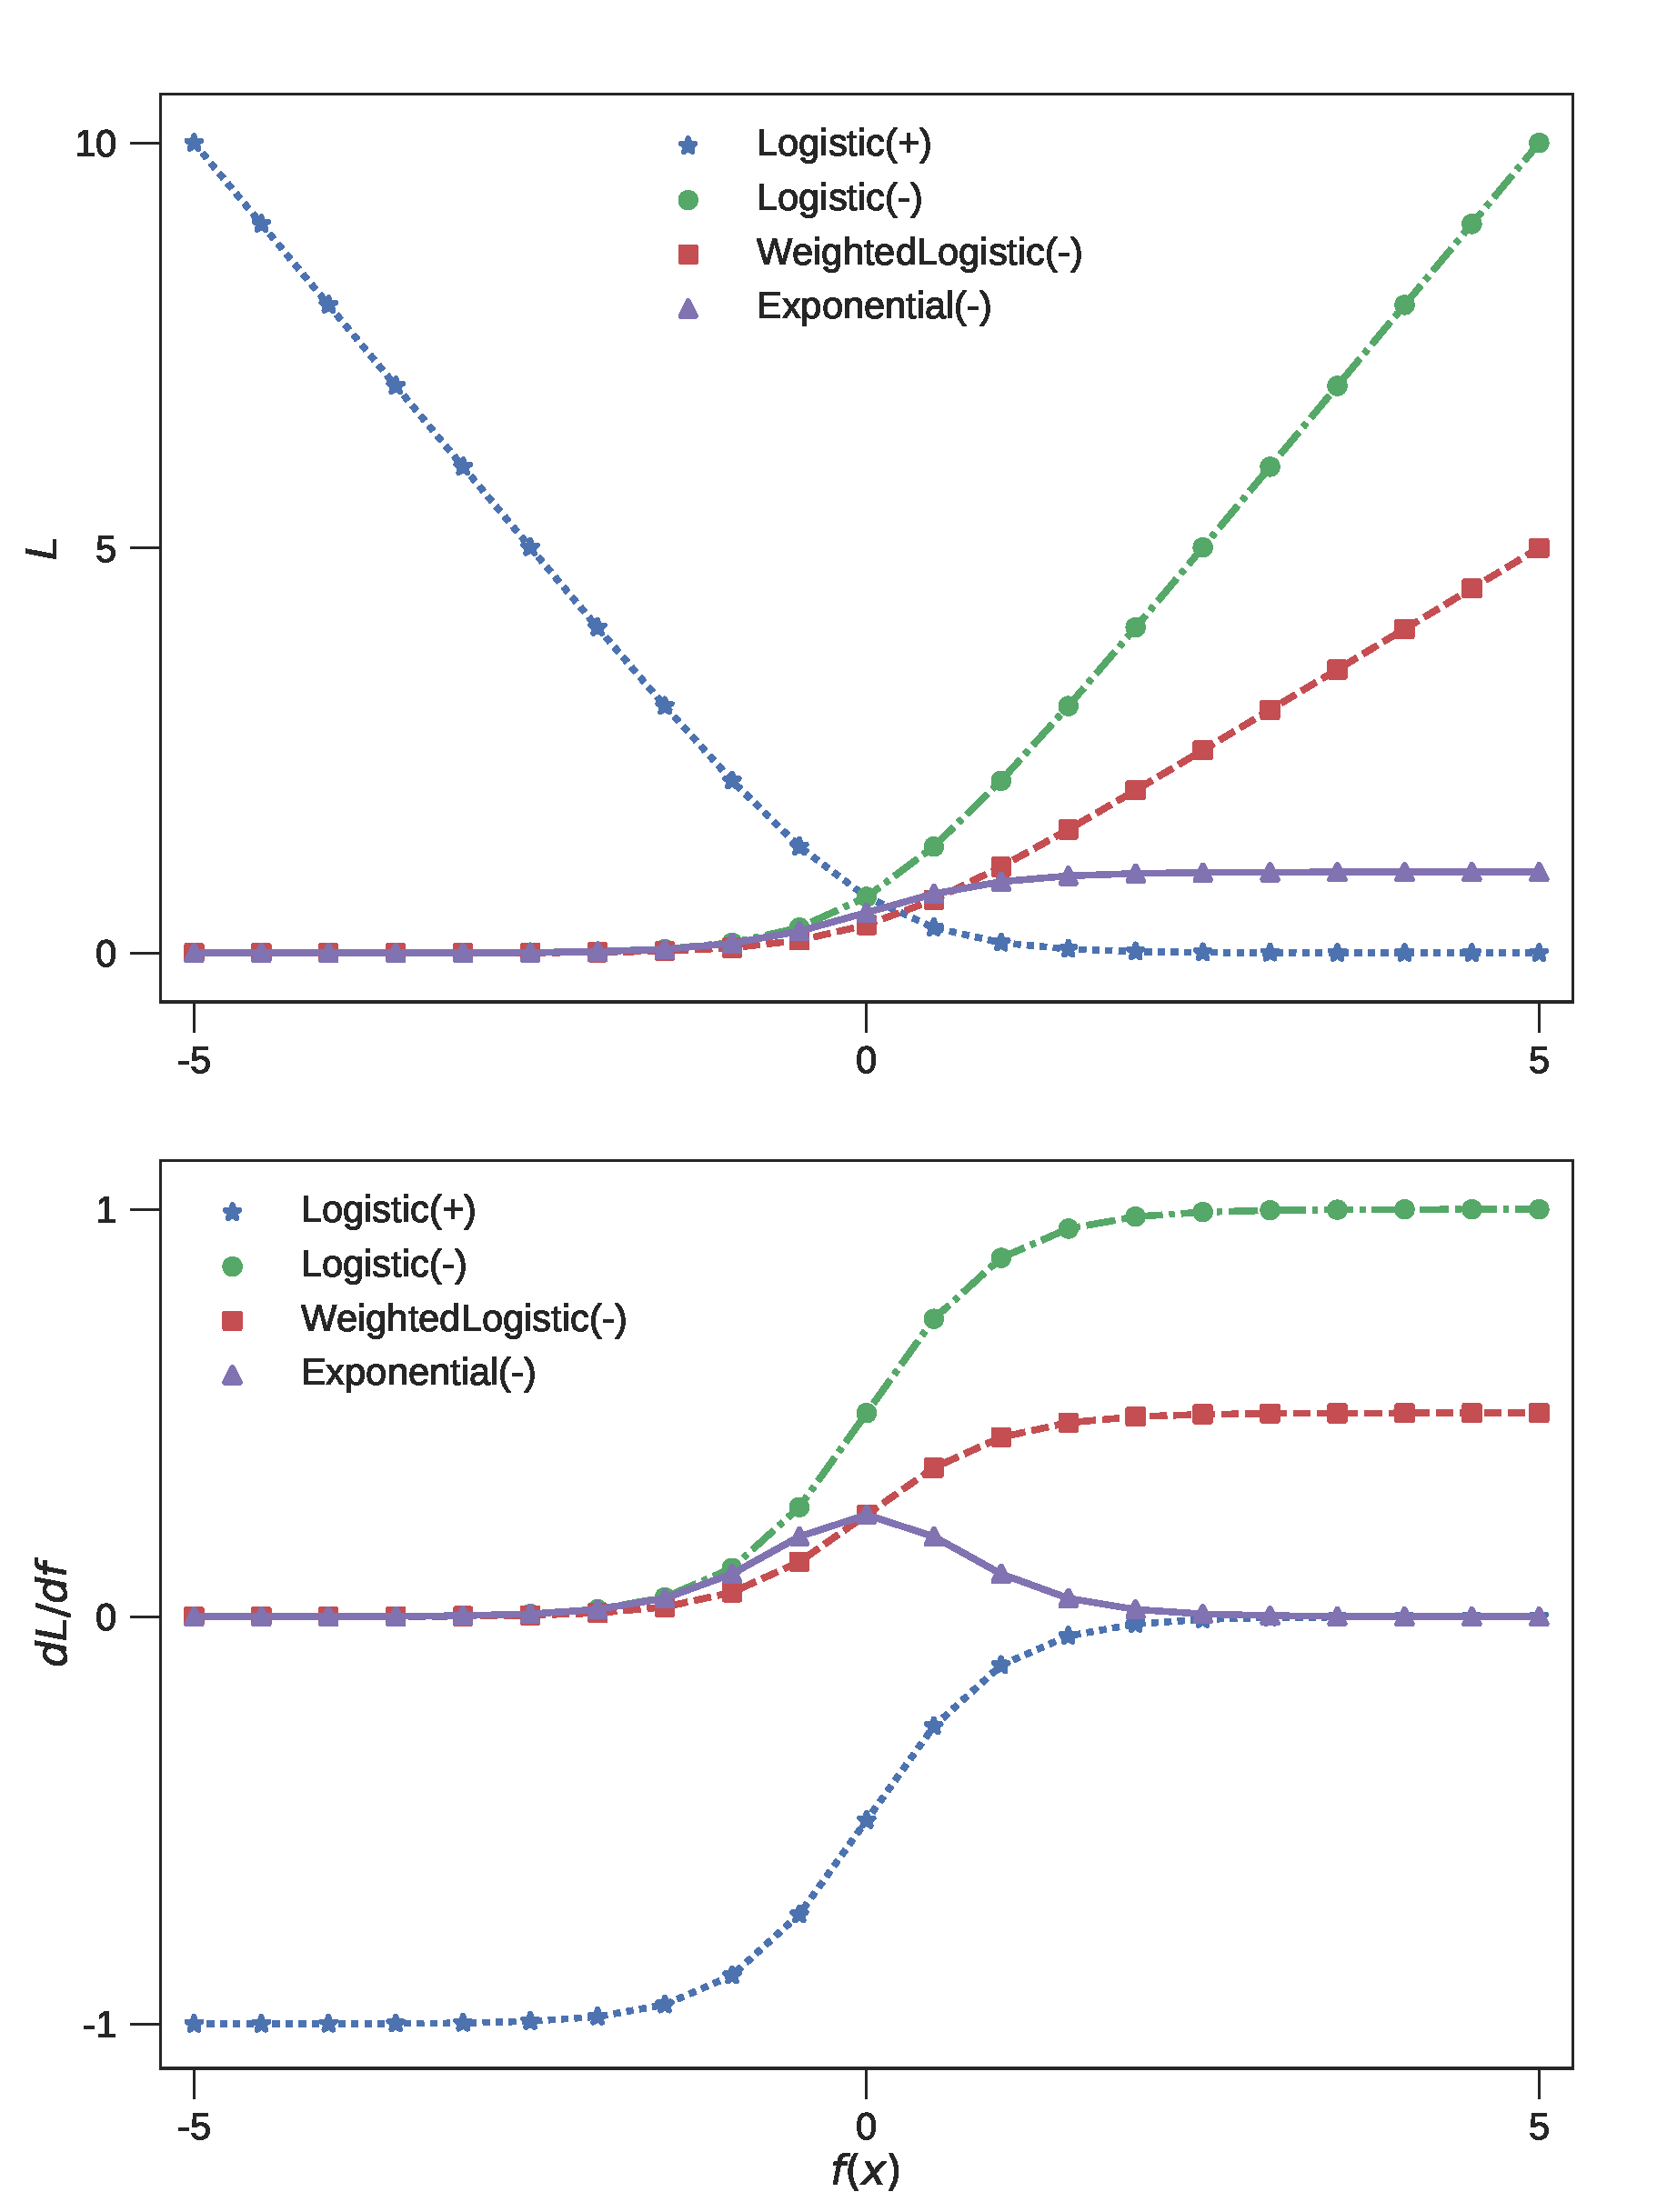
\includegraphics[width=1.05\linewidth]{img/losses}
\caption{The Logistic Loss, Weighted Logistic Loss, Exponential Loss and their derivatives with respect to logits.}
\label{fig:losses}
\end{figure}

%%%%%%%% FIGURE MOONS
\begin{figure*}
\begin{center}
% \fbox{\rule{0pt}{2in} \rule{.9\linewidth}{0pt}}
   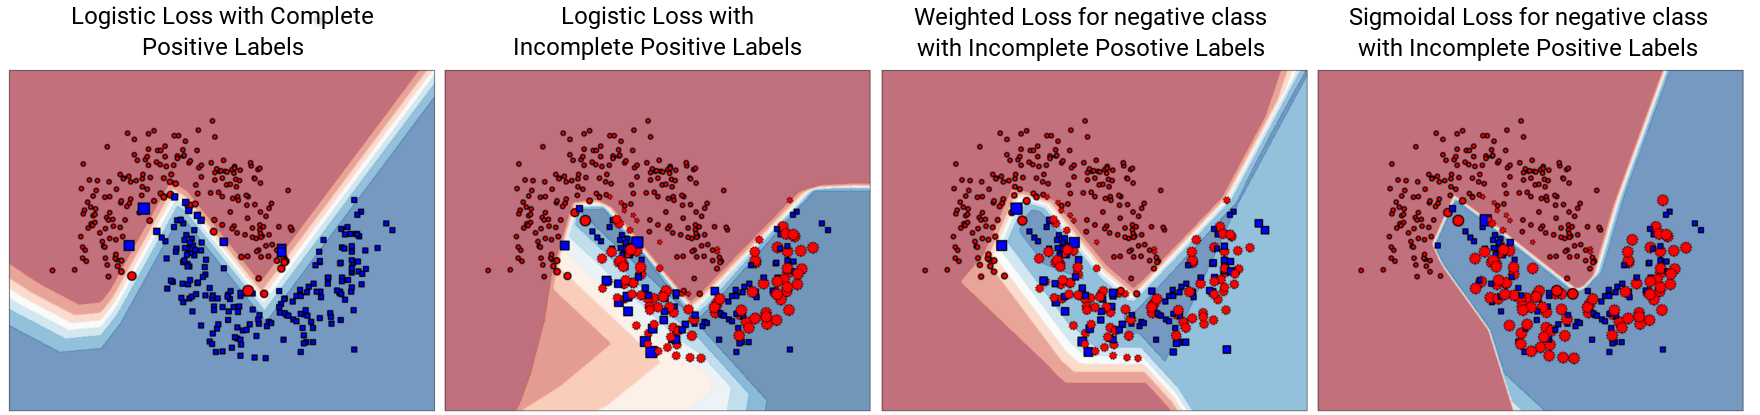
\includegraphics[width=0.95\linewidth]{img/moons.png}
\end{center}
   \caption{Decision boundaries for a 2-layer multilayer perceptron with different losses on a 2D moons dataset with unlabeled positive. Four hundreds samples per class were drawn randomly from two interleaving half circles with noises added with a minor standard deviation. A \textbf{red circle} indicates an example labelled as positive whilst a \textbf{blue square} indicates the example has a negative label. The \textbf{leftmost} figures have complete positive labels, meaning the positive and negative labels are all correct, whereas, in \textbf{the other figures} only half of the positives were correctly labelled and the rest were mixed with the negative samples. The \textbf{background colors} represent the probability for the area to be positive given by the classifier trained with the given samples and labels: \textbf{red} for high probability areas, \textbf{blue} for low probability areas and \textbf{white} for the class transition areas, i.e.decision boundaries. The \textbf{size of the markers} in the top row denotes the per-class normalized training losses and the \textbf{size of the markers} in the bottom row the per-class normalized derivatives w.r.t the output of the last layer for the trained Multilayer Perceptron (MLP) with the different losses.}
\label{fig:moons}
\end{figure*}


%%%%%%%% TEXT Bootstrapping
\paragraph{Minimum entropy regularization and bootstrapping objective}
\noindent
An alternative way of encouraging confident positive predictions is to introduce minimum entropy regularization\cite{grandvalet2005semi}.
Reed et al.\cite{reed2014training} proposed an emprical modification to softmax loss, a.k.a. the \textit{bootstrapping loss}, which can be used to learn with unlabeled examples:
% $$l_- = - \beta \log p(y=-1 \vert x) - (1-\beta) \sum_{j\in \{-1, +1\}} p(y=j \vert x) \log p(y=j \vert x)$$
\begin{equation*}
\resizebox{\columnwidth}{!}{
  $l_{\tilde{y_i}=-1} = - \beta \log p(y_i=-1 \vert x_i) - (1-\beta) \log p(y_i=\hat{y_i} \vert x_i)$
}
\end{equation*}
where $\hat{y} = argmax_{j\in\{-1,+1\}}p(y_i=j \vert x_i)$ is the model prediction and $0<\beta<1$.
The first term of the objective is a weighted logistic loss and the second term can be considered as a variation of minimum entropy regularization:
\begin{equation*}
  \begin{aligned}
    H = - \sum_{j\in\{-1,+1\}} p(y_i=j \vert x_i) \log p(y_i=j \vert x_i) \\
    \sim - \sum_{j\in\{-1,+1\}} \delta(y_i - \hat{y_i}) \log p(y_i=j \vert x_i)
  \end{aligned}
\end{equation*}
which intuitively encourages the model to make confident predictions\cite{grandvalet2005semi}.

%%%%%%%% TEXT Multiple classes
\paragraph{Multiclass PU learning}
\noindent \textit{This part should describe how to extend the losses for multiclass scenarios and the difficulty of having multiple positive classes.}
So far, we have been discussing modifications to the logistic loss for binary classification and segmentation.
Similiar modifications can be applied to softmax loss as well.
In a multi-class positive and unlabeled learning setup, $K>1$ positive classes are supposed to be distinguished from one negative class, whereas only part of the positive examples are labeled, and the others are not.
Softmax loss can be still used for positive classes because positive labels are reliable as long as they are given.
By contrast, the negatively labeled samples are a mix of samples assigned with true negative labels and false positive labels.
The weighted unlabeled logistic, exponential unlabeled loss and bootstrapping can be used for negative by simply replacing logistic function with softmax function as the activation function for logits.


%%%%%%%% TEXT Segmentation
\paragraph{From classification to segmentation}
\noindent \textit{This paragraph should highlight the problem of spatial independence assumption.}
Classification for each pixel is made independently when segmentation task is considered as per-pixel classification.
The objective modifications to alleviate the negative impact of unlabeled positive samples can be applied to classification for each pixel by assuming the probability of missing positive label for a pixel is independent of its neighbor pixels, which may not hold in practice.
For example, we stochastically flipped pixel labels for the whole segment, instead of individual pixel label, to synthesize incomplete segmentation errors in Section \ref{sec:robustness},
Even with annotation errors like under-segmented objects, the probability for a pixel to be unsegmented depends on its neighbor pixels.
We made a strong assumption of spatial independence for false negative labels for inexhaustive segmentation noises.
% This assumption allows to keep the problem simple and straightforward but we showed in Section \ref{subsec:pulearning} that this assumption become an issue to recover the whole unsegmented objects rather than individual pixels.
Future works maybe required to relax this assumption and make use of the spatial dependence of label noises to achieve higher mean intersection over union (mean IU) not only higher accuracy.

% It is nevertheless difficult to fit such a NNAR model directly because it is difficult to estimate of $p(e \vert x,y)$ with limited number of samples.
% An alternatie model is the \textit{noisy at random (NAR)} model in which the occurence of errors $e$ are independent to $x$ only on $y$: $p(\tilde{y} \vert y)p(y \vert x)$
% Such \textit{Noisy at random (NAR)}

%%%%%%%% TEXT Expontial loss FADE IN
\paragraph{Implementation details}
\noindent \textit{This paragraph should explain fade-in was introduced to avoid all-positive inital prediction;}
\noindent
The exponential loss for negative (unlabeled) examples saturates for very positive outputs, meaning that the confident positive prediction has little contribution to the total loss.
This can introduce problems at the beginning of the training procedure when the confident predictions are likely to be made at random.
Additionally, optimization could reach the plateau where the model made all positive predictions with high confidence.
Therefore, we introduced the exponential loss after training with the normal logistic/softmax loss for a few epochs.
We applied a similar ``fade-in'' mechanism to the bootstrapping objective as well because it also requires a non-random model for sufficiently trustworthy prediction $\hat{y}$.


%%%%%%%% TEXT Imbalanced
\noindent
\textit{This part should explain the influence of the imbalanced problem and how to overcome.}
\noindent
Another problem encountered in the PU learning setup is the class imbalance introduced by negatively labeled positive samples.
Even a balanced dataset can become imbalanced in the presence of false negative labels, especially if only a small portion of positive samples are correctly labeled.
We reweighed positive and negative samples based on their occurrences of the observed labels to alleviate the influence of imbalance for training.
Note that the class-weighted logistic loss reweighed the classes in addtion to this frequency balancing class weight.
